%%%%%%%%%%%%%%%%%%%%%%%%%%%%%%%%%%%%%%%%%%%%%%%%%%%%%%%%%%%%%%%%%%%%%%%%%%%%%%
% University of Bristol presentation theme based on the PowerPoint template
%
% Copyright (c) 2012, 2020 David A.W. Barton (david.barton@bristol.ac.uk)
% All rights reserved.
%
% The latest version of this theme can be found at
%   https://github.com/db9052/UoB-beamer-theme
%
% This is dual licensed under the MIT license and CC BY 4.0
%%%%%%%%%%%%%%%%%%%%%%%%%%%%%%%%%%%%%%%%%%%%%%%%%%%%%%%%%%%%%%%%%%%%%%%%%%%%%%
% \documentclass[aspectratio=169, handout]{beamer}
\documentclass[aspectratio=169]{beamer}
    % Possible aspect ratios are 16:9, 16:10, 14:9, 5:4, 4:3 (default) and 3:2
    % (Remember to remove the colon, i.e., 16:9 becomes the option 169) 

\usetheme{UoB}
% If lualatex is used then Rockwell, Latin Modern math, and Arial are used as
% per the UoB style (you need these fonts installed; they are installed by 
% default on Windows). If pdflatex is used then Concrete, Euler math, and 
% Helvetica are used as the closest alternatives.

% To use the Rockwell font in Overleaf, you will need to download a copy of
% the Truetype font (various websites appear to have it available for free -
% licensing is uncertain though) and put it in this folder with the name
% "Rockwell.ttf" and then change the compiler (under the menu) to LuaLaTeX.

\bibliographystyle{apalike}


\usepackage{tikz}
%\usetikzlibrary{shapes,arrows,positioning}
\usetikzlibrary{automata,arrows,positioning,calc}
\usetikzlibrary{shapes,snakes}

\usepackage{amsmath}
\usepackage{amssymb}
\usepackage{dsfont}

\usepackage{mathtools}
\newcommand{\defeq}{\vcentcolon=}
\newcommand{\eqdef}{=\vcentcolon}
\newcommand{\Var}{\text{Var}}

\DeclareMathOperator*{\argmax}{argmax} % thin space, limits underneath in displays
\DeclareMathOperator*{\argmin}{argmin}

%%%%%%%%%%%%%%%%%%%%%%%%%%%%%%%%%%%%%%%%%%%%%%%%%%%%%%%%%%%%%%%%%%%%%%%%%%%%%%
\title[Short Title]{Self-Tuning Spectral Clustering}
% \subtitle{Filtering, Smoothing \& Parameter Estimation}
\author{Sam Bowyer}
\institute{Statistical Methods 2}
\date{24th February 2023}

%%%%%%%%%%%%%%%%%%%%%%%%%%%%%%%%%%%%%%%%%%%%%%%%%%%%%%%%%%%%%%%%%%%%%%%%%%%%%%
% Lectures to include

% Lectures available (see \lecture commands below):
%   01: Introductory slides

\ifdefined\uselecture
  % Automatically generate specific lecture slides: run (lua/pdf)latex with
  % latex -jobname "slides-01" "\def\uselecture{01}\input{slides.tex}"
  % latex -jobname "handout-01" "\def\uselecture{01}\PassOptionsToClass{handout}{beamer}\input{slides.tex}"
  \expandafter\includeonlylecture\expandafter{\uselecture}
\else
  % Default lecture to output - comment out to get all lectures
  \includeonlylecture{01}
\fi

% Uncomment to get title slides for each lecture
% \AtBeginLecture{
%   \subtitle{\insertlecture}
%   \setcounter{framenumber}{0}
%   \begin{frame}
%     \titlepage
%   \end{frame}
% }

%%%%%%%%%%%%%%%%%%%%%%%%%%%%%%%%%%%%%%%%%%%%%%%%%%%%%%%%%%%%%%%%%%%%%%%%%%%%%%
% Start of the slides

\begin{document}

% Available frame options:
%   leftcolor, rightcolor: set the colour of the left or right panel
%   leftimage, rightimage: put a (cropped) image in the left or right panel
%   div: set the location of the divider between left and right panels
%   urlcolor: set the colour of the url

% Other commands available:
%   \logo{X}: choose the logo to display (logo, white logo, or black logo)
%   \urltext{X}: change the url for each slide

% All standard University of Bristol colours are available:
%   UniversityRed, CoolGrey, BrightAqua, BrightBlue, BrightOrange, BrightPurple,
%   BrightPink, BrightLime, DarkAqua, DarkBlue, DarkOrange, DarkPurple,
%   DarkPink, DarkLime

\begin{frame}[leftcolor=white,rightcolor=UniversityRed,div=0.8\paperwidth]
  \titlepage
\end{frame}

%%%%%%%%%%%%%%%%%%%%%%%%%%%%%%%%%%%%%%%%%%%%%%%%%%%%%%%%%%%%%%%%%%%%%%%%%%%%%%
\lecture{Lecture 1}{01}

\begin{frame}
\frametitle{Table of Contents}
\tableofcontents
\end{frame}

\section{1. Recap: Spectral Clustering}
%%%%%%%%%%%%%%%%%%%%%%%%%%%%%%%%%%%%%%%%%%%%%%%%%%%%%%%%%%%%
\begin{frame}{Basic Spectral Clustering Algorithm}
    To cluster $n$ data points $\{\mathbf{x}_i\}_{i=1}^n$ into $K$ clusters:
    \begin{enumerate}[<+->]
      \item Form the affinity/similarity matrix $W \in \mathbb{R}^{n \times n}$ where $W_{ij} = \exp\left(-\frac{d^2(\mathbf{x}_i, \mathbf{x}_j)}{\sigma^2}\right)$ for $i \neq j$ and $W_{ii} = 0$.
      \item Let $G$ be the diagonal matrix with $G_{ii} = \sum_{j=1}^n W_{ij}$ (the degree of $x_i$).
      Let $\tilde{L} \vcentcolon = G^{-1/2} W G^{-1/2}$ be the symmetric normalized Laplacian.
      \item Form the matrix $Z \in \mathbb{R}^{n \times K}$ by stacking the eigenvectors corresponding to the $K$ largest eigenvalues of $\tilde{L}$.
      % \item Re-normalise the rows of $Z$ to unit length, giving $Z' \in \mathbb{R}^{n \times K}$ where $Z_{ij}' = Z_{ij}/\left({\sum_{l=1}^K Z_{il}^2}\right)^{1/2}$.
      \item Cluster the rows of $Z$ using $K$-means: assign $x_i$ to cluster $k \in [K] \vcentcolon= \{1, \ldots, K\}$ if and only if row $i$ of $Z$ was assigned to cluster $k$.
    \end{enumerate}
    \cite{ng_spectral_2001}

\end{frame}

\section{2. Self-Tuning Spectral Algorithm}
%%%%%%%%%%%%%%%%%%%%%%%%%%%%%%%%%%%%%%%%%%%%%%%%%%%%%%%%%%%%
\begin{frame}{Parameters To Tune}
    \alert{Problem:} we have to choose $K$ and $\sigma$.
    \newline
    \pause

    \alert{Self-Tuning Spectral Clustering} \cite{zelnik-manor_self-tuning_2004} contributions:
    \begin{itemize}
      \item[(i)] Selection of the appropriate scale to analyse the data.
      \item[(ii)] Clustering data distributed at different scales.
      \item[(iii)] Clustering with irregular background clutter.
      \item[(iv)] Estimating the number of clusters.
    \end{itemize}
    \pause
    Selecting a suitable $\sigma$ will resolve (i)--(iii), whilst (iv) is just choosing $K$.
\end{frame}

\subsection{Selecting $\sigma$}
%%%%%%%%%%%%%%%%%%%%%%%%%%%%%%%%%%%%%%%%%%%%%%%%%%%%%%%%%%%%
\begin{frame}{Selecting $\sigma$}
    Note that $\sigma$ can be \alert{very} sensitive.
    \begin{figure}
      \centering
      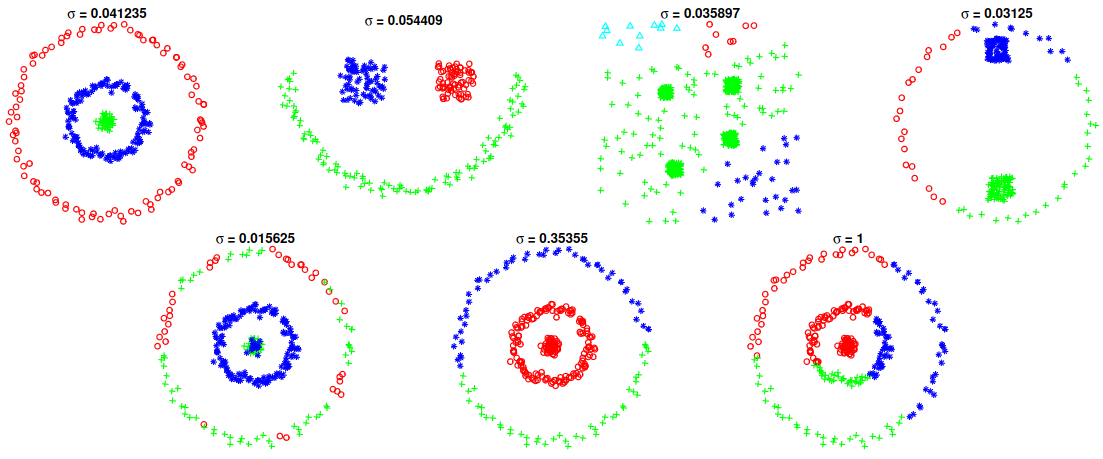
\includegraphics[scale=0.3]{sensitive_sigma.png}
      \caption{Fig. 1 from \cite{zelnik-manor_self-tuning_2004}.}
    \end{figure}
\end{frame}

%%%%%%%%%%%%%%%%%%%%%%%%%%%%%%%%%%%%%%%%%%%%%%%%%%%%%%%%%%%%
\begin{frame}{Local Scaling}
    Furthermore, different bandwidths $\sigma$ may be needed for different clusters which are distributed at different scales.
    So we introduce \alert{local scaling}:
    \pause
    \begin{enumerate}%[<+->]
      \item For each data point $\mathbf{x}_i$, define $\sigma_i = d(x_i, x_P)$, i.e. the distance from $x_i$ to its $P$th nearest neighbour, $x_P$. ($P=7$ suggested.)
      \pause
      \item The \textit{locally scaled} affinity matrix's non-diagonal entries are given by $\hat{W}_{ij} = \exp\left(-\frac{d^2(x_i, x_j)}{\sigma_i \sigma_j}\right)$.
    \end{enumerate}
    \pause
    \begin{figure}
      \centering
      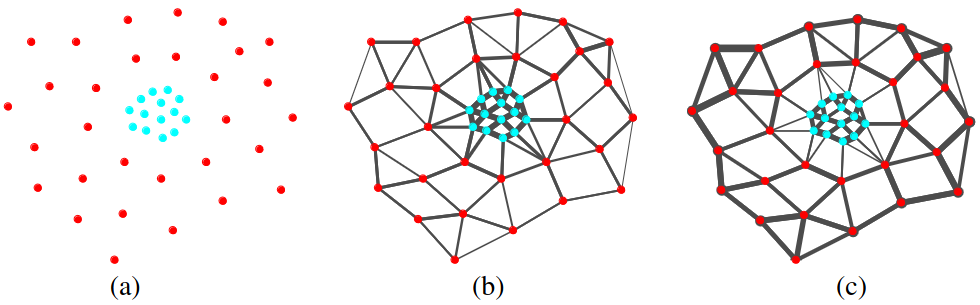
\includegraphics[scale=0.22]{local_scaling.png}
      \caption{Fig. 2 from \cite{zelnik-manor_self-tuning_2004}: (a) Input data; (b) unscaled affinity; (c) locally-scaled affinity (edge thickness represents weight).}
    \end{figure}
\end{frame}

\subsection{Selecting $K$}
%%%%%%%%%%%%%%%%%%%%%%%%%%%%%%%%%%%%%%%%%%%%%%%%%%%%%%%%%%%%
\begin{frame}{Selecting $K$}
    In the ideal case that there are some $K$ completely disconnected clusters (i.e. $\hat{W}_{ij} > 0$ if and only if $x_i$ and $x_j$ are in the same cluster), then the eigenvalues of $\tilde{L}$, given by $\lambda_1 \geq \lambda_2 \geq \cdots \geq \lambda_n$, will be such that:
    \[1 = \lambda_1 = \cdots = \lambda_K > \lambda_{K+1} \geq \cdots \geq \lambda_n \geq 0.\]
    
    This leads to the ``eigengap heuristic" for choosing $K$: choose $K$ to be the smallest integer such that $\lambda_{K} - \lambda_{K+1}$ is large.
    \newline\newline
    \pause
    However, with real, noisy data, the above may not hold (``lacks a theoretical justification" \cite{zelnik-manor_self-tuning_2004})---so instead of looking at the eigenvalues, we'll look further into the structure of $\tilde{L}$'s eigenvectors.

\end{frame}

%%%%%%%%%%%%%%%%%%%%%%%%%%%%%%%%%%%%%%%%%%%%%%%%%%%%%%%%%%%%
\begin{frame}{Analysing the Eigenvectors}
  In our ideal case (i.e. with $K$ completely disconnected clusters), $\tilde{L}$ is block diagonal, with each block $\tilde{L}^{(k)}$ corresponding to a cluster $k \in [K]$.
  \pause
  Therefore when we construct $Z \in \mathbb{R}^{n \times K}$ by stacking the eigenvectors of $\tilde{L}$ corresponding to the $K$ largest eigenvalues of $\tilde{L}$, we obtain
  \[Z = \begin{bmatrix}
    \mathbf{v}^{(1)} & \overrightarrow{\mathbf{0}} &\overrightarrow{\mathbf{0}} \\
    \overrightarrow{\mathbf{0}}  & \hdots &  \overrightarrow{\mathbf{0}} \\
    \overrightarrow{\mathbf{0}} & \overrightarrow{\mathbf{0}} & \mathbf{v}^{(K)}
  \end{bmatrix} \in \mathbb{R}^{n \times K}\]
  where $\mathbf{v}^{(k)}$ is the eigenvector corresponding to the largest eigenvalue (i.e. 1) of the submatrix $\tilde{L}^{(k)}$.
  
  % Each row $i$ of $Z$ has only one nonzero entry, lying in the column $j$ corresponding to $x_i$'s cluster.
  % Taking more than $K$ eigenvectors would result in more than one nonzero entry in some rows of $Z$, whilst taking fewer would result in some rows of $Z$ having no nonzero entries.

\end{frame}

%%%%%%%%%%%%%%%%%%%%%%%%%%%%%%%%%%%%%%%%%%%%%%%%%%%%%%%%%%%%
\begin{frame}{Analysing the Eigenvectors}
  % In our ideal case (i.e. with $K$ completely disconnected clusters), $\tilde{L}$ is block diagonal, with each block $\tilde{L}^{(k)}$ corresponding to a cluster $k \in [K] = \{1, \ldots, K\}$.
  % Therefore when we construct $Z \in \mathbb{R}^{n \times K}$ by stacking the eigenvectors of $\tilde{L}$ corresponding to the $K$ largest eigenvalues of $\tilde{L}$, we obtain
  \[Z = \begin{bmatrix}
    \mathbf{v}^{(1)} & \overrightarrow{\mathbf{0}} &\overrightarrow{\mathbf{0}} \\
    \overrightarrow{\mathbf{0}}  & \hdots &  \overrightarrow{\mathbf{0}} \\
    \overrightarrow{\mathbf{0}} & \overrightarrow{\mathbf{0}} & \mathbf{v}^{(K)}
  \end{bmatrix} \in \mathbb{R}^{n \times K}\]
  % where $\mathbf{v}^{(k)}$ is the eigenvector corresponding to the largest eigenvalue (i.e. 1) of the submatrix $\tilde{L}^{(k)}$.
  
  \begin{itemize}
    \item[1.] Each row $i$ of $Z$ has only one nonzero entry, lying in the column $j$ corresponding to $x_i$'s cluster---making the remaining task of cluster allocation trivial.
    \pause
    \item[2.] Taking more than $K$ eigenvectors would result in more than one nonzero entry in some rows of $Z$, whilst taking fewer would result in some rows of $Z$ having no nonzero entries.
  \end{itemize}
  \pause
  With noisy, non-ideal data the rows of $Z$ may have more than one nonzero entry, but there should hopefully be one entry significantly larger than the others.
  
  Assign $x_i$ to the cluster $k = \argmax_j Z_{ij}^2$.
\end{frame}

%%%%%%%%%%%%%%%%%%%%%%%%%%%%%%%%%%%%%%%%%%%%%%%%%%%%%%%%%%%%
\begin{frame}{A Problem With $Z$}
  % \newline\newline
  \alert{Problem:} The eigensolver we use may not return the $K$ eigenvectors of $\tilde{L}$ in the standard basis---it could return any set of orthonormal vectors spanning the same space as $Z$'s columns.
  \pause

  \alert{Solution:} Find the rotation matrix $R \in \mathbb{R}^{K \times K}$ that minimises the cost function
  \[J_K = \sum_{i=1}^n \sum_{j=1}^K \frac{\hat{Z}_{ij}^2}{\max_l (\hat{Z}_{il}^2)}\]
  where $\hat{Z} = Z R$ is the rotated matrix of eigenvectors.% and $M_i = \max_l \hat{Z}_{il}$.
  \pause
  \newline\newline
  Minimising this attempts to make the rows of $\hat{Z}$ as close to the standard basis as possible (i.e. with only one nonzero entry) and can be done via gradient descent (see \cite{zelnik-manor_self-tuning_2004} for details).
  
\end{frame}

%%%%%%%%%%%%%%%%%%%%%%%%%%%%%%%%%%%%%%%%%%%%%%%%%%%%%%%%%%%%
\begin{frame}{Selecting $K$ from $\hat{Z}$}
  Choosing some large $K'$ we can calculate the value of $J_K$ for all $K \in [K']$ efficiently as follows:
  \pause
  \begin{enumerate}
    \item Let $Z \in \mathbb{R}^{n \times 2}$ be the matrix of eigenvectors of $\tilde{L}$ corresponding to the two largest eigenvalues of $\tilde{L}$.
    \pause\item Find the rotation $R$ that minimises $J_K$ on $Z \in \mathbb{R}^{n \times 2}$ to obtain $\hat{Z}$.
    \pause\item Add the eigenvector corresponding to the next largest eigenvalue of $\tilde{L}$ as a column to $\hat{Z}$ and find the rotation $R$ that minimises $J_K$ for $K = 3$.
    \pause\item Repeat until we've found $J_{K'}$.
  \end{enumerate}
  \pause
  Finally, we choose $K_{\text{best}} = \argmin_{K \in [K']} J_K$.
  (Although, if several $K$s have very similar costs---e.g. within 0.01\% of each other---then choose the largest of these $K$s.)

  \end{frame}

%%%%%%%%%%%%%%%%%%%%%%%%%%%%%%%%%%%%%%%%%%%%%%%%%%%%%%%%%%%%
\begin{frame}{Cluster Allocation}
  Now that we have $K_{\text{best}}$, using the rotated matrix $\hat{Z} \in \mathbb{R}^{n \times K_{\text{best}}}$ we can allocate each data point $x_i$ to a cluster $k$ in one of two ways: 
  \pause 
  \begin{enumerate}[<+->]
    \item Assign $x_i$ to the cluster $k = \argmax_j \hat{Z}_{ij}^2$.
    \item As in the old algorithm, perform $K$-means on the rows of $\hat{Z}$ to find the clusters (this should converge fairly quickly since \alert{(1)} is likely to be a good initialisation).
    This is particularly useful for very noisy data.
  \end{enumerate}
\end{frame}

\subsection{Algorithm}
%%%%%%%%%%%%%%%%%%%%%%%%%%%%%%%%%%%%%%%%%%%%%%%%%%%%%%%%%%%%
\begin{frame}{Self-Tuning Spectral Clustering Algorithm}
  % To cluster $n$ data points $\{\mathbf{x}_i\}_{i=1}^n$:
  \begin{enumerate}[<+->]
    \item Compute the local scale $\sigma_i$ for each data point $x_i$.
    \item Form the locally scaled affinity matrix $\hat{W} \in \mathbb{R}^{n \times n}$ where $\hat{W}_{ij} = \exp\left(-\frac{d^2(\mathbf{x}_i, \mathbf{x}_j)}{\sigma_i \sigma_j}\right)$ for $i \neq j$ and $\hat{W}_{ii} = 0$. 
    \item Let $G$ be the diagonal matrix with $G_{ii} = \sum_{j=1}^n \hat{W}_{ij}$ (the degree of $x_i$) and $\tilde{L} \vcentcolon = G^{-1/2} \hat{W} G^{-1/2}$ be the symmetric normalized Laplacian.
    % \item Form the matrix $Y \in \mathbb{R}^{n \times K'}$ by stacking the eigenvectors of $\tilde{L}$ corresponding to the $K'$ largest eigenvalues of $\tilde{L}$ (for some large $K'$).
    \item For some large $K'$, form the matrix $Z \in \mathbb{R}^{n \times K'}$ by stacking the eigenvectors corresponding to the $K'$ largest eigenvalues of $\tilde{L}$ and use gradient descent to find the rotation matrix $R \in \mathbb{R}^{K' \times K'}$ that minimizes $J_{K'} = \sum_{i=1}^n \sum_{j=1}^{K'} (Z_{ij}^2 / \max_l Z_{il}^2)$. %M_i^2$ where $M_i = \max_j Z_i$.
    \item Choose $K_{\text{best}} = \argmin_K J_K$ (or largest such $K$ if several give very similar costs).
    \item Assign $x_i$ to cluster $k$ if and only if $\max_j Z_{ij}^2 = Z_{ik}^2$. 
    (Or, for very noisy data, use $K$-means to cluster the rows of $Z$ as in the standard algorithm.)
  \end{enumerate}
\cite{zelnik-manor_self-tuning_2004}
\end{frame}

\section{3. Experiments}
%%%%%%%%%%%%%%%%%%%%%%%%%%%%%%%%%%%%%%%%%%%%%%%%%%%%%%%%%%%%
\begin{frame}{}
    \begin{figure}
      \centering
      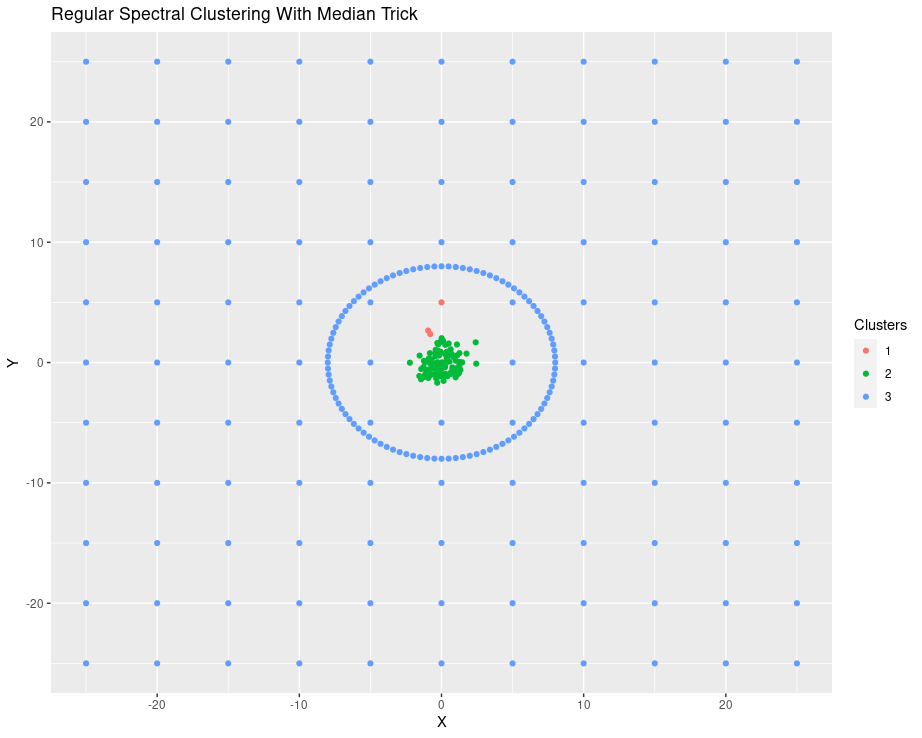
\includegraphics[width=0.8\textwidth]{code/regularSC.png}
      \caption{Iris dataset}
    \end{figure}
\end{frame}

%%%%%%%%%%%%%%%%%%%%%%%%%%%%%%%%%%%%%%%%%%%%%%%%%%%%%%%%%%%%
\begin{frame}{}
  \begin{figure}
    \centering
    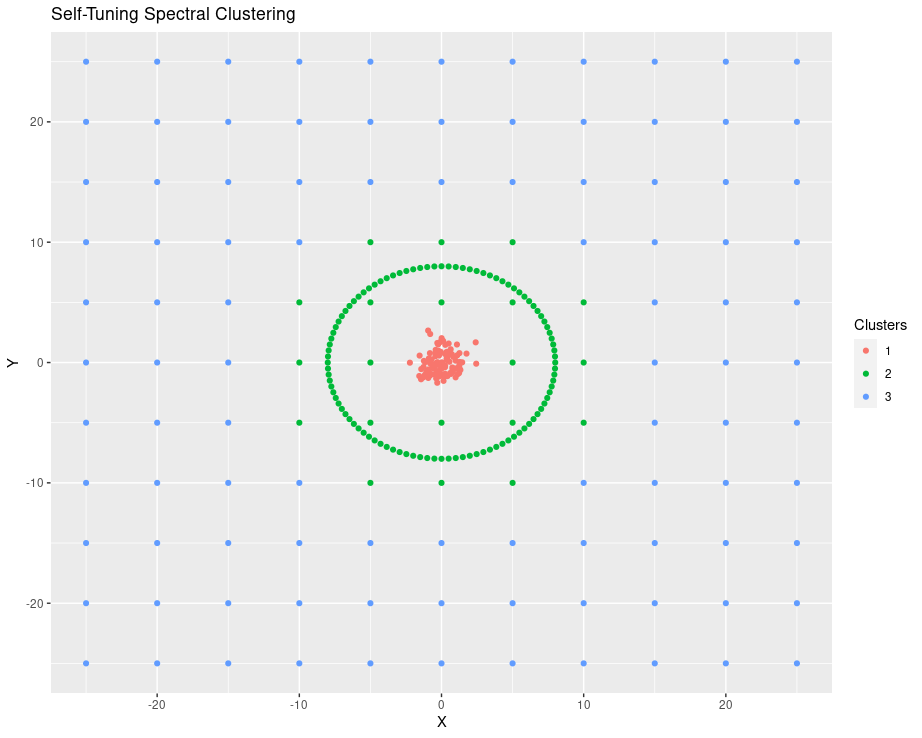
\includegraphics[width=0.8\textwidth]{code/STSC.png}
    \caption{Iris dataset}
  \end{figure}
\end{frame}

%%%%%%%%%%%%%%%%%%%%%%%%%%%%%%%%%%%%%%%%%%%%%%%%%%%%%%%%%%%%
\begin{frame}{Conclusion}
    \begin{itemize}
      \item Self-tuning spectral clustering allows us to determine suitable values of $\sigma$ and $K$ automatically.
      \item We do have to choose $P$ and $K'$, but these are much simpler to tune (and we can usually just set $K'$ to be `big enough' in some sense).
      \item The local scaling implemented to deal with $\sigma$ also allows us to perform clustering noisy, multi-scale data.
    \end{itemize}
\end{frame}

%%%%%%%%%%%%%%%%%%%%%%%%%%%%%%%%%%%%%%%%%%%%%%%%%%%%%%%%%%%%
\begin{frame}{References}
        \bibliography{refs.bib}
\end{frame}

%%%%%%%%%%%%%%%%%%%%%%%%%%%%%%%%%%%%%%%%%%%%%%%%%%%%%%%%%%%%
\begin{frame}{Thank you}
\centering
    Any questions?
\end{frame}

% %%%%%%%%%%%%%%%%%%%%%%%%%%%%%%%%%%%%%%%%%%%%%%%%%%%%%%%%%%%%
% \begin{frame}{Using Gradient Descent To Find Eigenvalue Rotations}
%   bhk;vjhv
%   \end{frame}

\end{document}

%%%%%%%%%%%%%%%%%%%%%%%%%%%%%%%%%%%%%%%%%%%%%%%%%%%%%%%%%%%%%%%%%%%%%%%%%%%%%%
